\documentclass{bioinfo}
\copyrightyear{2016} \pubyear{2016}

\usepackage{graphicx}
\usepackage{caption}
\usepackage{subfigure}


\access{Advance Access Publication Date: Day Month Year}
\appnotes{Databases and ontologies}

\begin{document}
\firstpage{1}

\subtitle{Databases and ontologies}

\title[RTCGA Family of R packages]{RTCGA - The Family of R Packages Integrating Data from The Cancer Genome Atlas Study}
\author[Marcin Kosi\'nski \textit{et~al}.]{Marcin Kosiński\,$^{\text{\sfb 1,2,}*}$, Witold Chodor\,$^{\text{\sfb 2}}$ and Przemys\l{}aw Biecek\,$^{\text{\sfb1,2}}$}
\address{$^{\text{\sf 1}}$Faculty of Mathematics and Information Science, Warsaw University of Technology, 00-662 Warsaw, Poland and \\
$^{\text{\sf 2}}$Faculty of Mathematics, Informatics, and Mechanics, University of Warsaw, City, 02-097 Warsaw, Poland.}

\corresp{$^\ast$To whom correspondence should be addressed.}

\history{Received on XXXXX; revised on XXXXX; accepted on XXXXX}

\editor{Associate Editor: XXXXXXX}

\abstract{\textbf{Summary:} The following article presents \textbf{RTCGA} software package and a family of \textbf{R} \citep{rpackage} packages with data from The Cancer Genome Atlas Project (TCGA) study \citep{broad}. TCGA is a comprehensive and coordinated effort to accelerate our understanding of the molecular basis of cancer through the application of genome analysis technologies, including large-scale genome sequencing [1]. We converted selected datasets from this study into few separate packages that are hosted on \citep{Bioconductor}. These R packages make selected datasets easier to access and manage. Datasets in \textbf{RTCGA} packages are large and cover complex relations between clinical outcomes and genetic background. These packages will be useful for at least three audiences: biostatisticians that work with cancer data; researchers that are working on large scale algorithms; teachers that are presenting data analysis method on real data problems \\
\textbf{Availability:} \textbf{RTCGA} family of R packages is freely available at http://rtcga.github.io/RTCGA/ and from
the  Bioconductor  project  at  http://bioconductor.org/packages/RTCGA/ .\\
\textbf{Contact:} \href{m.p.kosinski@gmail.com}{m.p.kosinski@gmail.com}}


\maketitle

\section*{Motivation}
The Cancer Genome Atlas (TCGA) Data Portal provides a platform for researchers to search, download, and analyze data sets generated by TCGA. It contains clinical information, genomic characterization data, and high level sequence analysis of the tumor genomes [1]. 

TCGA data is available through Firehose Broad GDAC portal [1]. One can select cancer type (cohort) and data type (e.g. clinical, RNA expression, methylation, ..) and download a `tar.gz` file with compressed data. 

When working with many cancer types we find this approach burdensome:

\begin{itemize}
\item If one requires to download datasets containing e.g. information about genes' expressions for all available cohorts types (TCGA collected data for more than 30 various cancer types) one would have to go through the click-to-download process many times, which is inconvenient and time-consuming.
\item Clinical datasets from TCGA project are not in a standard tidy data format, which is: one row for one observation and one column for one variable. They are transposed which makes work with that data burdensome. That becomes more onerous when one would like to investigate
many clinical datasets.
\item Datasets containing information on some data types (e.g. gene's mutations) are not in one easy-to-handle file. Every patient has it's own file, what for many potential researchers may be an impassable barrier. 
\item Data governance for many datasets for various cohorts saved in different folders with strange (default after untarring) names may be exhausting and uncomfortable for researchers that are not very skilled in data management or data processing.
\end{itemize}
For these reasons we prepared selected datasets from the TCGA project in an easy to handle and process way and embed them in 9 separate R packages. All packages can be installed from BioConductor.
\section*{Examples}

\begin{figure*}
	\begin{center}
	\subfigure[The workflow of \textbf{RTCGA} family of software and data R packages. \textbf{RTCGA} consists of auxiliary functions: \texttt{infoTCGA()} and \texttt{checkTCGA} that enable to find out metadata about datasets and dates of their release provided by TCGA. Data download section consists of \texttt{downloadTCGA()} function that allows to download every dataset from TCGA study and \texttt{readTCGA()} function that enables to read (most popular) data into the tidy format. It is possible to use \texttt{installTCGA()} function to install, prepared in tidy format, most popular data types from TCGA that are included in data packages. Datasets in \textbf{RTCGA} data packages can be converted to Bioconductor format (\texttt{ExpressionSet, GRanges}) with \texttt{convertTCGA()} function. Effects of functions designed to manipulate and visualize \textbf{RTCGA} data are presented on subfigures (b)-(e).]{
	\includegraphics[width=0.99\linewidth]{figures/RTCGA_workflow_ver3}}
	
	\subfigure[Kaplan-Meier \citep{kaplanmeier} estimates of survival curves and risk set table for \textbf{Breast invasive carcinoma (BRCA)} and \textbf{Ovarian serous cystadenocarcinoma (OV)} cohorts divided on \textbf{TP53} mutations. The effect of \texttt{survivalTCGA()}, \texttt{mutationsTCGA()} and \texttt{kmTCGA()} functions.]{
	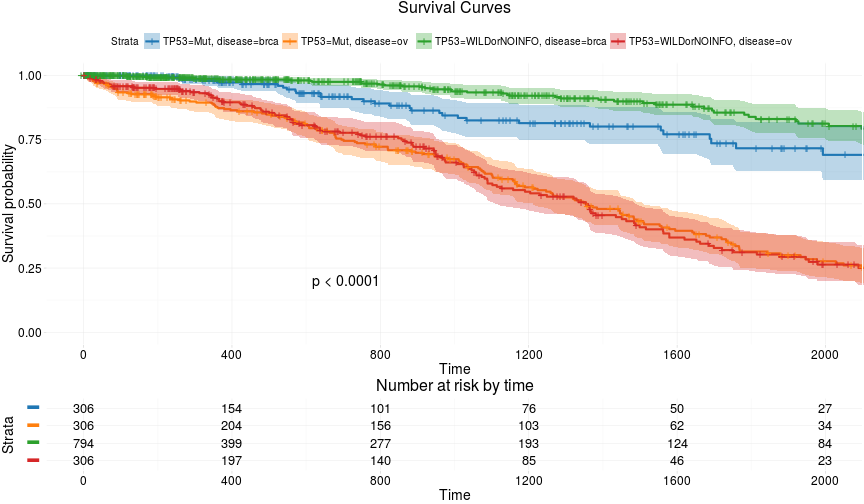
\includegraphics[width=0.48\linewidth]{figures/km}}
\hspace{5pt}
	\subfigure[Plot of Principal Component Analysis \citep{krzanowski2000principles} performed for genes expressions (RNASeq) for \textbf{Breast invasive carcinoma (BRCA)}, \textbf{Head and Neck squamous cell carcinoma (HNSC)} and \textbf{Ovarian serous cystadenocarcinoma (OV)} cohorts. The effect of \texttt{expressionsTCGA()} and \texttt{pcaTCGA()} functions.]{
	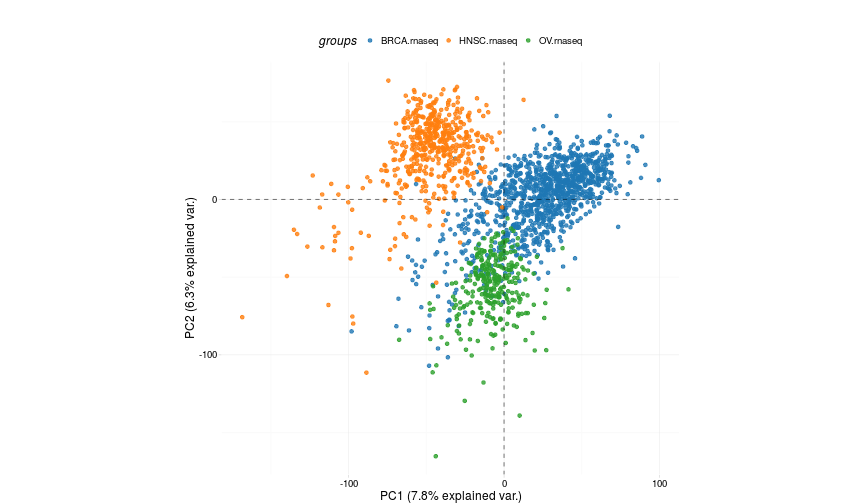
\includegraphics[width=0.48\linewidth]{figures/pca}}
	\subfigure[Boxplots \citep{10.2307/2683468} of logarithm of \textbf{MET} gene expression (RNASeq) for \textbf{Adrenocortical carcinoma (ACC)}, \textbf{Bladder urothelial carcinoma (BLCA)}, \textbf{Breast invasive carcinoma (BRCA)} and \textbf{Ovarian serous cystadenocarcinoma (OV)} divided on mutations in gene \textbf{TP53}. The effect of \texttt{expressionsTCGA()} and \texttt{boxplotTCGA()} functions.]{
	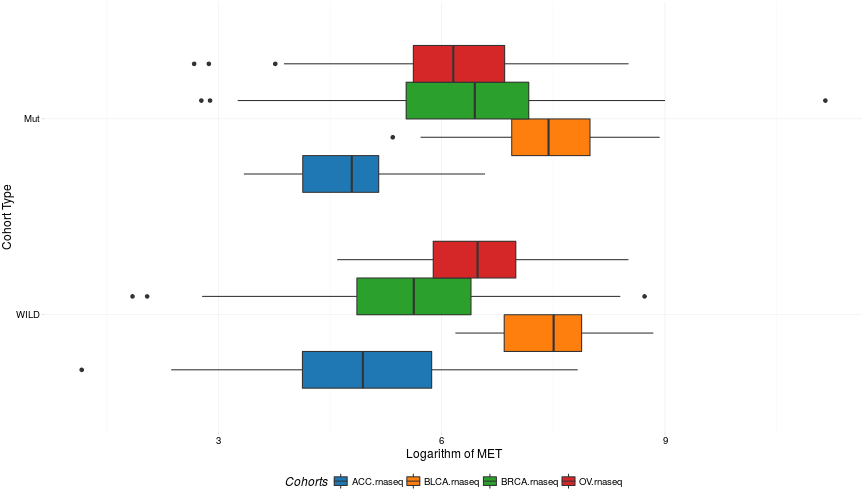
\includegraphics[width=0.48\linewidth]{figures/boxplots}}
\hspace{5pt}
	\subfigure[Heatmap \citep{10.2307/2291215} presenting medians of \textbf{ZNF500} gene for \textbf{Adrenocortical carcinoma (ACC)}, \textbf{Bladder urothelial carcinoma (BLCA)}, \textbf{Breast invasive carcinoma (BRCA)} and \textbf{Ovarian serous cystadenocarcinoma (OV)} divided on \textbf{MET} gene quantiles. The effect of \texttt{expressionsTCGA()} and \texttt{heatmapTCGA()} functions.]{
	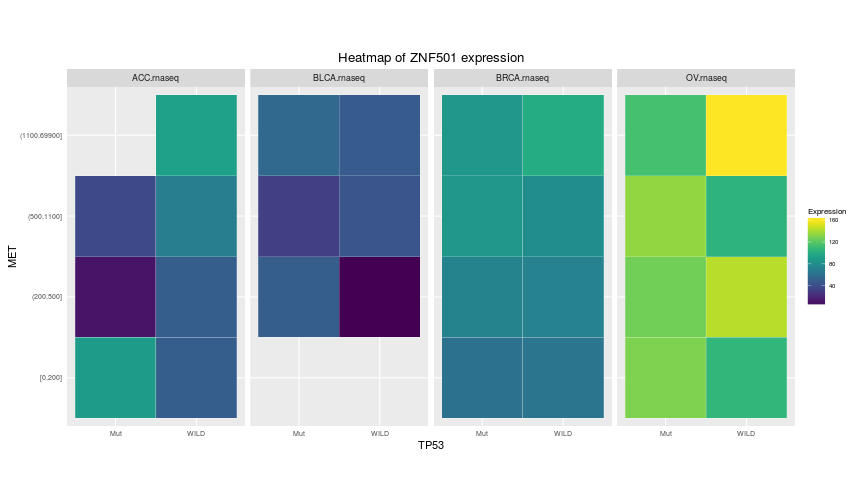
\includegraphics[width=0.48\linewidth]{figures/heatmap}}	
	\end{center}
\caption{The workflow of \textbf{RTCGA} family of software and data R packages and effects of functions designed to manipulate and visualize \textbf{RTCGA} data. }
\label{fig:RTCGA_workflow_ver3}
\end{figure*}

\ \\ \ \\

\section*{Acknowledgements}

Text Text Text Text Text Text  Text Text.  \citealp{Boffelli03} might want to know about  text
text text text\vspace*{-12pt}

\section*{Funding}

This work has been supported by the... Text Text  Text Text.\vspace*{-12pt}

\bibliographystyle{natbib}
%\bibliographystyle{achemnat}
%\bibliographystyle{plainnat}
%\bibliographystyle{abbrv}
%\bibliographystyle{bioinformatics}
%
%\bibliographystyle{plain}
%
\bibliography{bibarticle}


\end{document}
